\chapter{Permutations of \ch{(CrFeMnNi)Si2}}
\label{sec:permutations}

Up until this point we have looked in detail at the high-entropy silicide \ch{(CrFeMnNi)Si2} and associated SQSs. However these structures are just the center of a larger quasi-ternary phase diagram consisting of the different possible distributions of elements Thus there exists many more permutations of this particular composition of a high-entropy silicide. In this section, we aim to expand our search of this diagram by generating SQSs slightly away from eqvimolar distribution of 3d elements. In table (bellow) we list the mean total energy and magnetic moment per atom with standard deviation and the enthalpy of formation of 4 permutations of the \ch{(CrFeMnNi)Si2} alloy. Ideally the permutations would differ only by one element, but the TDEP implementation insist in also reducing Nickel to stay consistent with the 48 atom supercell. 

\begin{table}[h!]
%\centering
\hskip-2.5cm\begin{tabular}{@{}cccccc@{}}
\toprule
       & \multicolumn{2}{c}{Total energy/atom (eV)} & Enthalpy of formation (eV) & \multicolumn{2}{c}{Final magnetic moment ($\mu_B$)} \\ \midrule
\ch{Cr3Fe3Mn7Ni3Si32} & - 6.6947  & 0.0040 & -11.9586  & 0.1375  & 0.0186     \\
\ch{Cr5Fe5Mn3Ni3Si32} & - 6.6705  & 0.0030 & -11.1991  & 0.1127  & 0.0223     \\
\ch{Cr5Fe3Mn5Ni3Si32} & - 6.6852  & 0.0041 & -10.5200  & 0.1375  & 0.0456     \\
\ch{Cr3Fe5Mn5Ni3Si32} & - 6.6801  & 0.0036 & -12.6426  & 0.0937  & 0.0209     \\
\ch{Cr3Fe3Mn3Ni7Si32} & - 6.3921  & 0.0078 & -10.9614  & 0.0159  & 0.0101 \\ \bottomrule
\end{tabular}
\caption{Mean and stadard deviation of the total energy and magnetic moment per atom, plus enthalpy of formation of the listed mean energies (\ch{FeSi2}).}
\end{table}

The first result of table .. we make notice of is that the stability, as evaluated by the enthalpy of formation can be increased beyond the eqvimolar composition. This is accomplished in two distinct permutations, one with increments to  manganese relative to the other TM, and the other by reduction of chromium. Moreover the two respective permutations lie on the opposite side of the magnetic scale. The large magnetic moment of the manganese rich permutation and the low magnetic moment in the chromium poor permutation is very much in line with the observations made in the previous section. Recalling that in the magnetic moment in the eqvimolar composition was largely attributed to manganese and chromium atoms in the lattice. Thus increments to manganese or reduction of chromium would following impact the magnetic moment as in the two permutations. For this reason, additionally the permutation \ch{Cr5Fe3Mn5Ni3Si32} where the nonmagnetic elements is reduced and the magnetic elements are increased ,is equally magnetic. We however find no direct relation between stability and magnetism as his particular permutation is the least stable. An important property of table 8.5 is that the listed values are the mean value of the observed property for 5 distinct SQSs of the same permutation. For example we notice that while the highest magnetic moment in the first permutation is associated with the most stable SQS (from total energy considerations). The least stable supercell show the highest magnetic moment in \ch{Cr5Fe3Mn5Ni3Si32}. 

The respective band gap of the permutations (with PBE) can be seen in table ... Compared to the previous case, we find most SQSs of the permutations to exhibit a half-metallic character. 

\begin{table}[H]
\centering
\begin{tabular}{@{}ccccc@{}}
\toprule
                                                     &   & Spin up (eV) & Spin down (eV) & Total (eV) \\ \midrule
\multicolumn{1}{c|}{\multirow{5}{*}{\textbf{\ch{Cr3Fe3Mn7Ni3Si32}}}}   & A & 0.3390                & 0                       & 0                   \\
\multicolumn{1}{c|}{}                                & B & 0.4745                & 0                       & 0                   \\
\multicolumn{1}{c|}{}                                & C & 0.1342                & 0                       & 0                   \\
\multicolumn{1}{c|}{}                                & D & 0.1950                & 0.0063                  & 0.0063              \\
\multicolumn{1}{c|}{}                                & E & 0.4211                & 0                       & 0                   \\ \midrule
\multicolumn{1}{c|}{\multirow{1}{*}{\textbf{\ch{Cr5Fe5Mn3Ni3Si32}}}}   & D & 0.0674                & 0.0413                  & 0.0372              \\ \midrule
\multicolumn{1}{c|}{\multirow{5}{*}{\textbf{\ch{Cr5Fe3Mn5Ni3Si32}}}} & A & 0.2082                & 0                       & 0                   \\
\multicolumn{1}{c|}{}                                & B & 0.4053                & 0                       & 0                   \\
\multicolumn{1}{c|}{}                                & C & 0.4659                & 0                       & 0                   \\
\multicolumn{1}{c|}{}                                & D & 0.0843                & 0.0121                  & 0.0121              \\
\multicolumn{1}{c|}{}                                & E & 0.3008                & 0                       & 0                   \\ \midrule
\multicolumn{1}{c|}{\multirow{4}{*}{\textbf{\ch{Cr3Fe5Mn5Ni3Si32}}}} & A & 0.3922                & 0                       & 0                   \\
\multicolumn{1}{c|}{}                                & C & 0.1285                & 0                       & 0                   \\
\multicolumn{1}{c|}{}                                & D & 0.2595                & 0.1004                  & 1.004               \\
\multicolumn{1}{c|}{}                                & E & 0.3591                & 0.1003                  & 0.0848              \\ \midrule
\multicolumn{1}{c|}{\multirow{1}{*}{\textbf{\ch{Cr3Fe3Mn3Ni7Si32}}}} & - & -                & -                      & -                   \\ \bottomrule
\end{tabular}
\caption{Total and spin dependent band gap of 4 permutations of CFMN (fesi2) with PBE GGA calculation. The structures that are excluded from this list either failed in calculations, or does not show any band gap.<}
\end{table}

From table ..  we see that likewise to the stability and magnetization also the band gap changes in the different directions. To some degree we find positive results of the band gap in each direction, but we see particularly that permutations rich in manganese provide very encouraging results. This is made clear from the fact that \ch{Cr3Fe3Mn7Ni3Si32}, \ch{Cr5Fe3Mn5Ni3Si32} and \ch{Cr3Fe5Mn5Ni3Si32} all include amounts of manganese higher than the eqvimolar composistion and all associated SQSs show at least strong half-metalic charachter or semiconducting. On the other side \ch{Cr5Fe5Mn3Ni3Si32} is the sole permutation with less manganse and correspondingly show the least sign of a band gap. Moreover the relative stability of the SQSs give further merit to the proposition. In the first permutation we find that the highest total energy is associated with SQS B, which as seen in table .. exhibit the largest spin up band gap of the particular permutation. Furthermore the two semiconducting SQSs in the last permutation is the two most stable arrangements. Reversely, in the manganese-poor permutation we find that the sole semiconducting SQS is the second least stable of that compound. Lastly, the opposite is the case is true in the third permutation. Despite the total energy not varying tremendously between SQSs of the same permutation, as seen by the standard deviation in table .., the continuing trend between stability and band gap is a promising result to report.

In figure 8.12 we plot the projected density of states around $E_F$ of the 4 permutations. Note that away from the Fermi energy the projected density of states is analogous to the parent compound, see appendix ..

\begin{figure}[H]
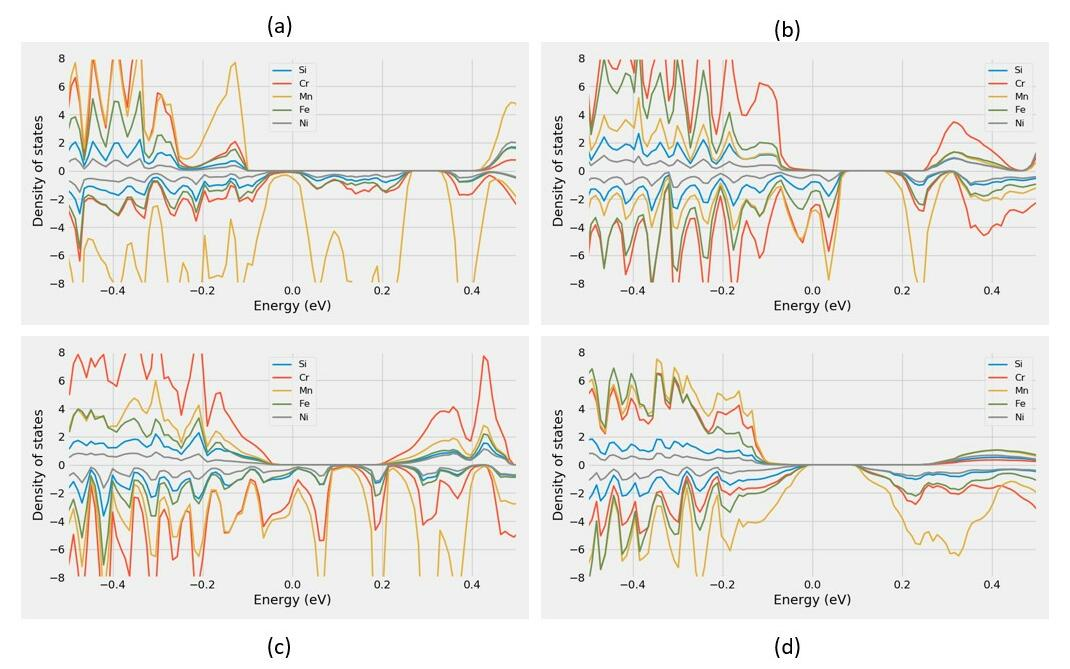
\includegraphics[width=\linewidth]{results/fesi2/permutations/perm_LDOS_crop.jpg}
\caption{Projected density of states of (a) \ch{Cr3Fe3Mn7Ni3Si32} (SQS B), (b) \ch{Cr5Fe5Mn3Ni3Si32} (SQS C), (c) \ch{Cr5Fe3Mn5Ni3Si32} (SQS A), (d) \ch{Cr3Fe5Mn5Ni3Si32} (SQS D)}
\end{figure}

The above figures is based on the most stable SQS in each permutation, as will the analysis. Thus the features of these figures does not necessarily represent the complete set of SQSs of the permutation. As experienced in table 8.6 and previous examples in this project, the band gap and properties of each permutation can vary between SQSs. But given that the structures came out on top in terms of total energy means that they are the most probable configuration of the real alloy, hence also the features of that supercell. 

With that said, the plotted PDOSs in figure 8.12 clearly illustrate the characteristics shown in table 8.6. We see clear indication of a spin up band gap in \ch{Cr3Fe3Mn7Ni3Si32} (a) and \ch{Cr5Fe3Mn5Ni3Si32} (c), and a total band gap in \ch{Cr3Fe5Mn5Ni3Si32} (d). Not so clear is that the density of states of \ch{Cr5Fe5Mn3Ni3Si32} (b) contain very small nonzero values at $E_F$ and the unoccupied states is shifted very slightly above the Fermi energy, prohibiting an otherwise clear band gap. In figure 8.13 the total density of states of SQS D and E of this permutation is shown, the above point is seen also in SQS E, where the "band gap" is shifted above $E_F$.
 
\begin{figure}[H]
	\begin{subfigure}{.5\textwidth}
		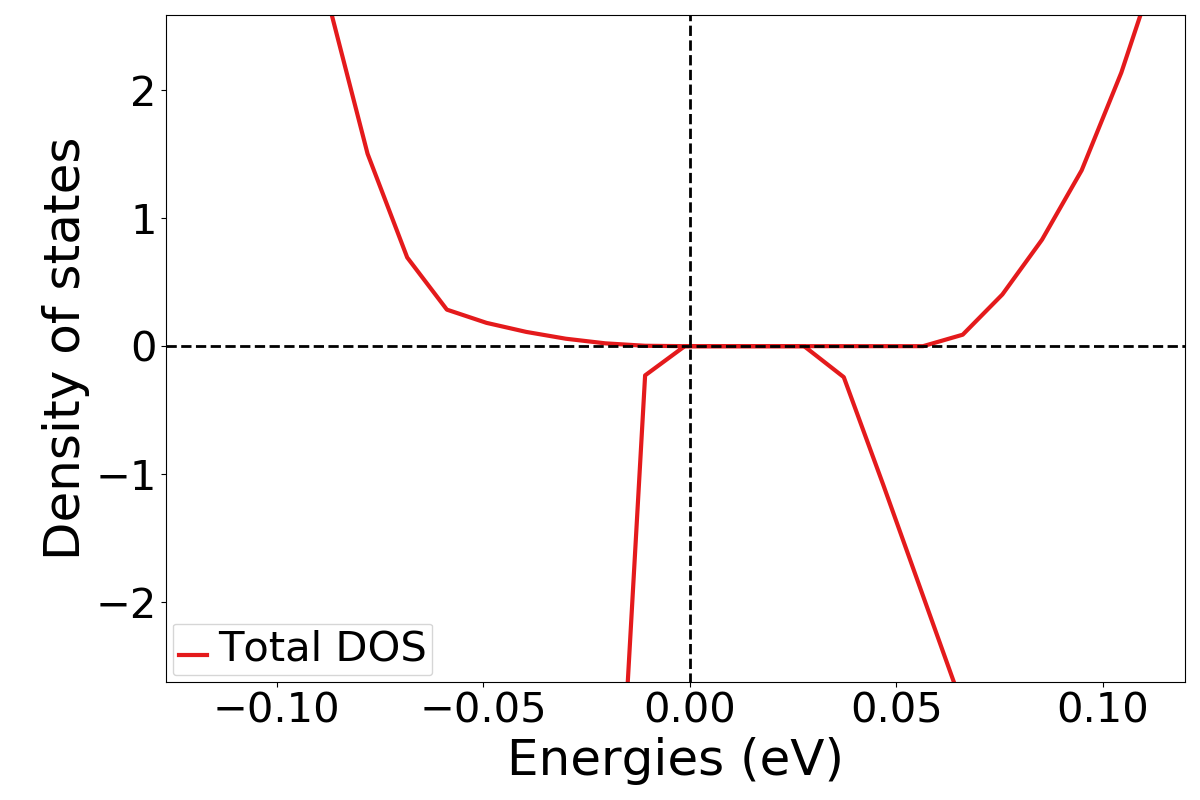
\includegraphics[width=\textwidth]{results/fesi2/permutations/mnni3_DOS.png}
		\caption{SQS D}
	\end{subfigure}
	\begin{subfigure}{.5\textwidth}
		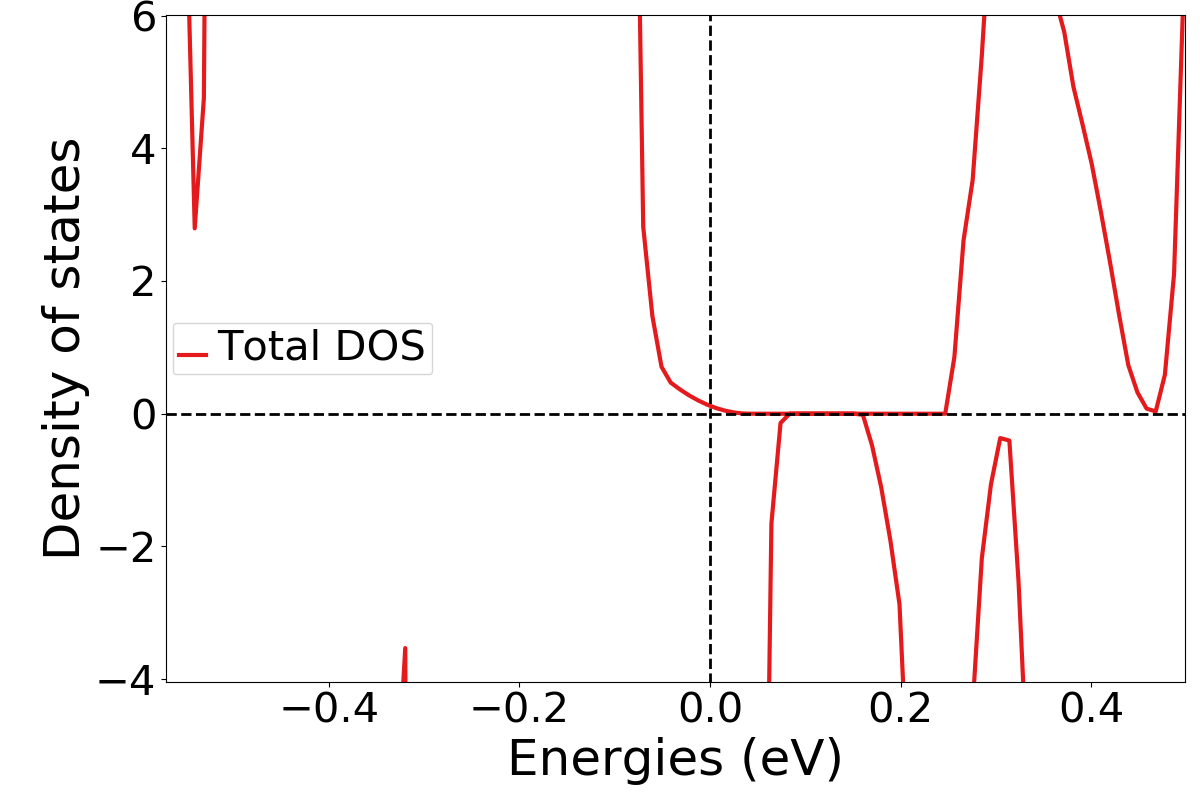
\includegraphics[width=\textwidth]{results/fesi2/permutations/mnni3_DOS_E.png}
		\caption{SQS E}
	\end{subfigure}
	\caption{Density of states around $E_F$ of SQS D and E \ch{Cr5Fe5Mn3Ni3Si32}}
\end{figure}


In figure 8.6 we saw that electrons from manganese atoms in particular was a key contributor as to why the spin down channel of \ch{(CrFeMnNi)Si2} was metallic in the stable supercell D. This is also largely the case in the permutations shown above in figure 8.12.    
 
The proportion of manganese atoms in the alloy seems to offer a very positive effect on the band gap in spin up, but is often detrimental to spin down. This is seen in figure 8.12 (a) and (c) for \ch{Cr3Fe3Mn7Ni3Si32} and \ch{Cr5Fe3Mn5Ni3Si32} respectively, that both contain increased amounts of manganese. By reducing the number of Mn as in (b) we still find that the Mn electrons plague the states at $E_F$ in spin down. In analog we see from (b) and (c) that also Cr negatively impacts to the band gap especially in spin up. The sole permutation with clear evidence of a spin down gap is from the chromium poor permutation plotted in (d). Also in this structure we see that the effects of Mn around $E_F$ is dampened in comparison to the other permutations, despite containing relatively increased amounts of Mn to the eqvimolar alloy.  

\begin{figure}[H]
	\centering
	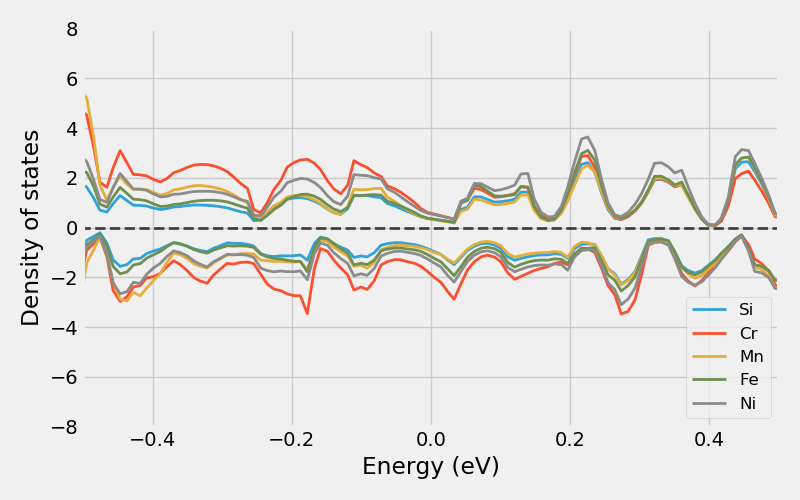
\includegraphics[width=.6\textwidth]{results/fesi2/permutations/ni7_PDOS.png}
	\caption{Projected density of states of \ch{Cr3Fe3Mn3Ni7Si32} around $E_F$}
\end{figure}

An important property of these results is that because each permutation alters simultaneous elements, interpreting and relating the results to a particular alteration is challenging. For example, is the result of the \ch{Cr5Fe3Mn5Ni3Si32} permutation a consequence of less Fe or increments to both Cr and Mn? Furthermore is the exaggerated band gap in spin up of \ch{Cr3Fe3Mn7Ni3Si32} a product of increasing manganese or reducing the other elements. From the comparatively large gaps in spin up of \ch{Cr3Fe3Mn7Ni3Si32} and \ch{Cr3Fe5Mn5Ni3Si32} and the more present Cr states in spin up in the Cr rich permutations we here conclude that the band gap is related to lessening of chromium, more so than other effects. Despite of this we generally find positive results regarding most of the permutations as seen in table 8.6, the exception to this \ch{Cr3Fe3Mn3Ni3si32}. This particular permutation in opposition to the others in this section increases the proportion of Ni at the cost of the other 3d elements. The projected density of states is displayed in figure [REF]. From both this structure, but also the PDOS of \ch{Cr3Fe3Mn7Ni3Si32} we see that reducing chromium does not always improve the band gap. It's clear that the \ch{Cr3Fe5Mn5Ni3Si32} alloy manage to strike a balance of distribution that results in a specific interplay between the 3d elements. For this reason we more closely investigate the properties of this structure, the probability distribution of SQS D (highest stability) is plotted bellow in figure 8.15.

\begin{figure}[H]
	\centering
	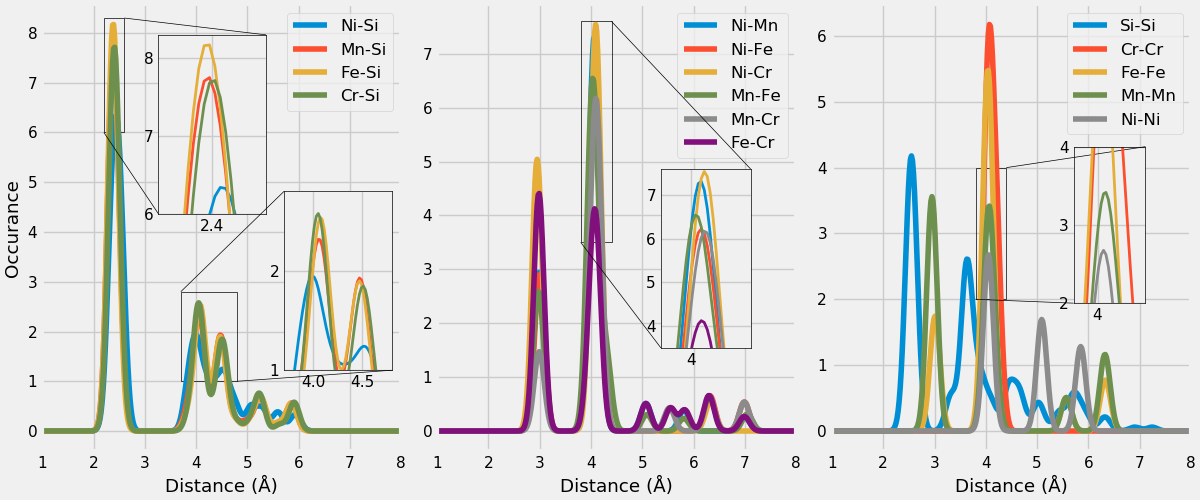
\includegraphics[width=\textwidth]{results/fesi2/permutations/_crni3_D_PDF.png}
	\caption{Probability distribution functions to \ch{Cr3Fe5Mn5Ni3Si32} SQS D, \textbf{Maybe make larger}}
\end{figure}

\textbf{Comment figure \\}

\textbf{Add some figures from HSE06?}
In this segment of the project we scarcely applied the more advanced functionals SCAN and HSE06, in part to both the uncertainties mentioned in the previous section and the computational cost of the methods. However we did perform such calculations (HSE06) to further investigate the nature of the listed semiconducting SQSs. Both the manganese rich and poor semiconductors are validated with the HSE06 functional and find wider band gaps of 0.17 eV (0.57 and 0.26 in up and down) in \ch{Cr3Fe3Mn7Ni3Si32} SQS D, and 0.22 eV (0.77 eV in spin up) in \ch{Cr5Fe5Mn3Ni3Si32} SQS D. On the opposite side, the very narrow band gap in \ch{Cr5Fe3Mn5Ni3Si32} vanishes with HSE06 calculations. For the two stable semiconductors found in \ch{Cr3Fe5Mn5Ni3Si32}, simulations with the HSE06 functional resulted in a half-metal with a spin up of 0.53 eV for SQS D, and a total band-gap of 0.27 eV for E, where the spin-up gap is 0.73 eV wide
. \textbf{Comparing to table 8.6 we observe that ..}. \textbf{As for the SCAN functional ...} 

\textbf{Conclusion this section \\}
